%**************************************************************
% CAPITOLO 2
%**************************************************************
\chapter{Il quadro strategico}
\label{cap:ilquadrostrategico}

\section{Strategie aziendali di stage}

L'azienda The White Dog s.r.l. accoglie e offre l'attività di stage per due principali motivi:

\begin{itemize}
	\item \textbf{Sperimentazione su progetti innovativi:} data la forte propensione alla ricerca dell'azienda, esistono numerosi campi che essa vorrebbe esplorare ma che a causa di altri progetti più prioritari e scarsità di tempo non può studiare. Offre quindi allo studente universitario un progetto di ricerca e sviluppo su tecnologie innovative ed interessanti, non pretendendo alcun risultato da subito inseribile nel mercato. Questo permette allo studente di vivere l'esperienza dello stage in piena libertà e serenità, riuscendo così a portare un notevole valore aggiunto personale che l'azienda è ben felice di accogliere;
	\item \textbf{Valutazione dello stagista:} l'azienda è in continua crescita e necessita di nuovo personale preparato e soprattutto capace di lavorare in costante sintonia col gruppo. Lo stage universitario permette all'azienda di scoprire persone che soddisfano questi due importanti requisiti per una futura assunzione.
\end{itemize}

Da parte sua The White Dog s.r.l. offre molto agli stagisti. I tutor aziendali supportano lo studente per tutto il periodo lavorativo, consigliandolo sia per quanto riguarda il piano di lavoro, sia sulle tecnologie da utilizzare sia effettuando proficue discussioni in vista della relazione finale. Allo studente viene offerto un ambiente di lavoro accogliente e strumenti aggiornati e all'avanguardia, supportandolo anche economicamente prevedendo un rimborso spese.

\section{Il progetto di stage proposto}

Il progetto propostomi nasce dalla costante volontà aziendale di ricercare nuove metodologie di interazione da proporre agli utenti dei suoi \textit{e-commerce} in ottica \textit{omni-channel}. Il modello \textit{omni-channel} si sta lentamente ma inesorabilmente affermando come principale modello di \textit{retailing}\ped{\hyperlink{ret}{G}} a livello globale e si basa sulle seguenti caratteristiche:

\begin{itemize}
	\item Concezione e management unitario della distribuzione;
	\item Processi basati sull'interazione, comunicazione e interdipendenza tra i \textit{team} dedicati ai singoli canali;
	\item Approccio dinamico al consumatore, che richiede un monitoraggio in tempo reale delle evoluzioni dei comportamenti di acquisto e delle risposte alle iniziative promosse;
	\item Predisposizione di adeguati strumenti IT e marketing in grado di sfruttare ed assecondare il fenomeno della cross-canalità dei processi di acquisto;
	\item Impatto competitivo decisivo delle scelte organizzative e di investimento nell'IT e nel marketing digitale;
	\item Impiego di indicatori di prestazioni e di sistemi di \textit{monitoring} adeguati al nuovo contesto.
\end{itemize}

Questo significa, da parte delle aziende, offrire un'unica \textit{customer experience} capace di rispondere in modo adeguato alle aspettative del consumatore omnicanale che si informa sui prodotti in mobilità, li prova e li sperimenta in negozio per poi acquistarli in loco o online. In termini pratici, questo si implementa costruendo un unico profilo del consumatore, immagazzinandovi dati sulle ricerche da lui effettuate, sulle scelte e sui dati personali immessi per poi sfruttarli in ogni tipologia di \textit{store}, sia digitale che fisico. \\
La realtà virtuale si pone nella strategia \textit{omni-channel} come punto di connessione tra \textit{store} digitale e fisico, permettendo all'utente di esplorare il negozio nella sua totalità e di osservarne i prodotti esposti da più angolazioni o indossati da modelli o manichini, nel caso dei capi di abbigliamento, il tutto con un alto livello di definizione. 
Nasce così l'idea di un \textit{e-commerce VR}, progetto in grado di colmare, in parte, quel divario che da sempre ha distanziato \textit{store} virtuale e negozio fisico.

\label{Omni-channel}
\begin{figure}[ht]
	\begin{center}
		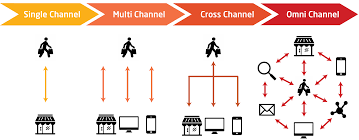
\includegraphics[scale=0.47]{omni-channel}
		\caption{Schema rappresentativo della differenze tra \textit{single-channel}, \textit{multi-channel}, \textit{cross-channel} e \textit{omni-channel}. Immagine tratta dal sito dell'azienda ON THE MARK: \url{http://on-the-mark.com/omnichannel-organization-designs-biggest-test/}}
	\end{center}
\end{figure}
\FloatBarrier

L'obbiettivo di stage è, dunque, un'esplorazione tecnologica nel campo della \textit{virtual reality}\ped{\hyperlink{vr}{G}}. Il progetto mira ad arrivare ad un prototipo di \textit{virtual showroom} dove poter esplorare ed interagire con i prodotti e permetterne l'acquisto. \\
Il progetto era stato inizialmente diviso in due parti, per due differenti studenti:
\begin{itemize}
	\item La prima parte riguardava la progettazione e realizzazione del movimento in uno spazio 3D ed interazione con gli oggetti;
	\item La seconda parte trattava, invece, la progettazione e realizzazione di un'interfaccia di presentazione del prodotto, con integrazione al processo di acquisto mediante l'uso di sistemi \textit{cloud} esterni.
\end{itemize}
Purtroppo, nessun altro studente oltre a me ha aderito al progetto, dunque abbiamo ritenuto opportuno rivisitare l'obbiettivo di stage. Dopo una riunione effettuata prima dell'inizio dello stage con il mio tutor aziendale, abbiamo deciso di mantenere intatti tutti gli obiettivi di ricerca, abbassando il livello qualitativo richiesto. Questo perché lo scopo ultimo di questo stage non era sviluppare un'applicazione o un servizio immediatamente vendibile, ma di studiare le potenzialità e i limiti di questa nuova tecnologia. Questa volontà è stata dettata anche dal fatto che il \textit{team} aziendale inizialmente non aveva alcuna certezza che la tecnologia \textit{VR}\ped{\hyperlink{vr}{G}} fosse applicabile al mondo \textit{e-commerce}.

\subsection{Piano di lavoro proposto}

\subsubsection{Piano temporale}

In accordo col tutor aziendale, la durata massima dello stage è stata fissata a 320 ore, divise in 8 settimane lavorative di 5 giorni, 8 ore al giorno. \\
Il piano lavorativo è stato dunque pianificato per settimana nel seguente modo:

\begin{itemize}
	\item \textbf{Settimana 1:} settimana dedicata completamente alla ricerca, per colmare il \textit{deficit} culturale personale e aziendale sulle tecnologie \textit{VR}\ped{\hyperlink{vr}{G}}. Le attività principali previste sono: analisi dei requisiti funzionali del sistema da sviluppare e studio delle tecnologie e linguaggi disponibili riguardanti la realtà virtuale;
	
	\item \textbf{Settimana 2:} in base ai risultati ottenuti nella prima settimana, viene richiesta una scelta dell'hardware da utilizzare e un \textit{framework}\ped{\hyperlink{fw}{G}} di sviluppo, testandoli con un primo prototipo di scena 3D;
	
	\item \textbf{Settimana 3:} previste attività di raffinamento della scena 3D, progettazione e sviluppo degli oggetti e loro comportamento nello spazio 3D. Viene creato così un primo prototipo di \textit{user interaction};
	
	\item \textbf{Settimana 4:} previste attività di progettazione e sviluppo integrazione tra sistema \textit{VR}\ped{\hyperlink{vr}{G}} e \textit{e-commerce}. Progettazione di \textit{user interaction} per la fruizione dei contenuti provenienti dall'\textit{e-commerce};
	
	\item \textbf{Settimana 5:} settimana dedicata all'approfondimento di \textit{user interaction} e del comportamento degli oggetti nell'ambiente virtuale;
	
	\item \textbf{Settimana 6:} previste attività di studio e prototipazione del possibile processo d'acquisto all'interno dell'ambiente virtuale;
	
	\item \textbf{Settimana 7:} la settima settimana rappresenta una \textit{milestone} importate per il progetto: conclusione del prototipo e relativa documentazione, raggiungendo così gli obbiettivi minimi;
	
	\item \textbf{Settimana 8:} l'ultima settimana viene dedicata completamente allo studio del modello emergente \textit{omni-channel}\ped{\hyperlink{oc}{G}} e come la realtà virtuale possa estendere questo modello. Vengono così raggiunti gli obbiettivi massimi.
\end{itemize}

\subsubsection{Piano metodologico}
	
Assieme al tutor aziendale, abbiamo fin da subito concordato la mia presenza durante l'orario d'ufficio, permettendo così un interazione intensa e costante. \\
Il lavoro di ricerca e sviluppo che ho effettuato è stato totalmente autonomo, con giornaliere interazioni con il personale solo per raccogliere e analizzare la documentazione, requisiti e \textit{feedback} sull'andamento del progetto. \\
Le revisioni di progetto sono avvenute secondo la seguente metodologia:

\begin{itemize}
	\item Riunione breve di 15 minuti ogni mattina;
	\item Riunione di 1 ora alla fine di ogni settimana come analisi retrospettiva.
\end{itemize}

Alle revisioni, oltre a me, hanno partecipato:

\begin{itemize}
	\item \textbf{Valentino Baraldo}, \textit{cloud engineer} e tutor aziendale. Oltre a svolgere il compito di tutor aziendale, mi ha supportato sulla progettazione architetturale del progetto e sull'utilizzo del servizio \textit{API Gateway} di \textit{Amazon Web Services}\footnote[1]{\url{https://aws.amazon.com/it/}};
	\item \textbf{Francesco Paggin}, \textit{front-end developer}. Ha supervisionato il mio lavoro grafico nell'ambiente di sviluppo \textit{Unity}\footnote[2]{\url{https://unity3d.com/}}.
\end{itemize}  

\subsubsection{Piano tecnologico}

Inizialmente lo \textit{stack} tecnologico propostomi riguardava solamente l'hardware che l'azienda aveva acquistato per questo progetto, senza alcun vincolo software. I dispositivi che permettevano la sperimentazione \textit{VR}\ped{\hyperlink{vr}{G}} erano:

\begin{itemize}
	\item \textbf{Oculus Rift Development kit 2:} visore per la realtà virtuale per uso desktop. Possiede uno schermo Samsung OLED 2160x1200 pixel (1080x1200 per occhio), con un \textit{refresh rate} a 90 Hz e un ampio angolo di visione a 110 gradi. Dotato di accelerometro, giroscopio, magnetometro e \textit{tracking} posizionale a 360 gradi. Viene accoppiato ad una telecamera infrarossi per il rilevamento di profondità, assieme a 40 emettitori infrarossi all'interno dell'\textit{headset}. Monta due lenti in alta definizione possedendo 6 gradi di libertà di rotazione;
	
	\item \textbf{Samsung Gear VR:} visore per la realtà virtuale per uso \textit{mobile}. Possiede: accelerometro, giroscopio e sensore di prossimità, permettendo un campo visivo di 96 gradi. Il visore incorpora inoltre un'interfaccia utente fisica: \textit{touch pad}, tasto indietro e tasto per il volume. Necessita l'inserimento di uno \textit{smartphone} Samsung a partire dalla versione \textit{Galaxy S6};
	
	\item \textbf{Google Cardboard:} con il termine \textit{Google Cardboard} non si intende specificare un particolare visore per la realtà virtuale prodotto fisicamente da \textit{Google}, ma un insieme di linee guida suggerite da questa per costruire un dispositivo a basso costo per l'uso \textit{mobile}. Non possiede accelerometro, giroscopio o sensore di prossimità, è solo un semplice "occhiale" che permette la visione stereoscopica. Ogni visore \textit{Cardboard}, dunque, necessita l'inserimento di uno \textit{smartphone} che supporti applicazioni \textit{VR}\ped{\hyperlink{vr}{G}}. \\ 
	In azienda erano presenti due visori che implementavano tali linee guida: \textit{Unofficial Cardboard} e \textit{Tera VR Box};
	
	\item \textbf{Leap Motion:} piccola periferica USB  progettata per essere posta su una scrivania reale rivolta verso l'alto. Usando 2 telecamere e 3 LED infrarossi essa osserva un'area approssimativamente a forma di semisfera di circa un metro. E' progettata per identificare dita o oggetti simili come una penna, con una precisione di 0,01 mm. 
\end{itemize}

\label{Gear VR}
\begin{figure}[ht]
	\begin{center}
		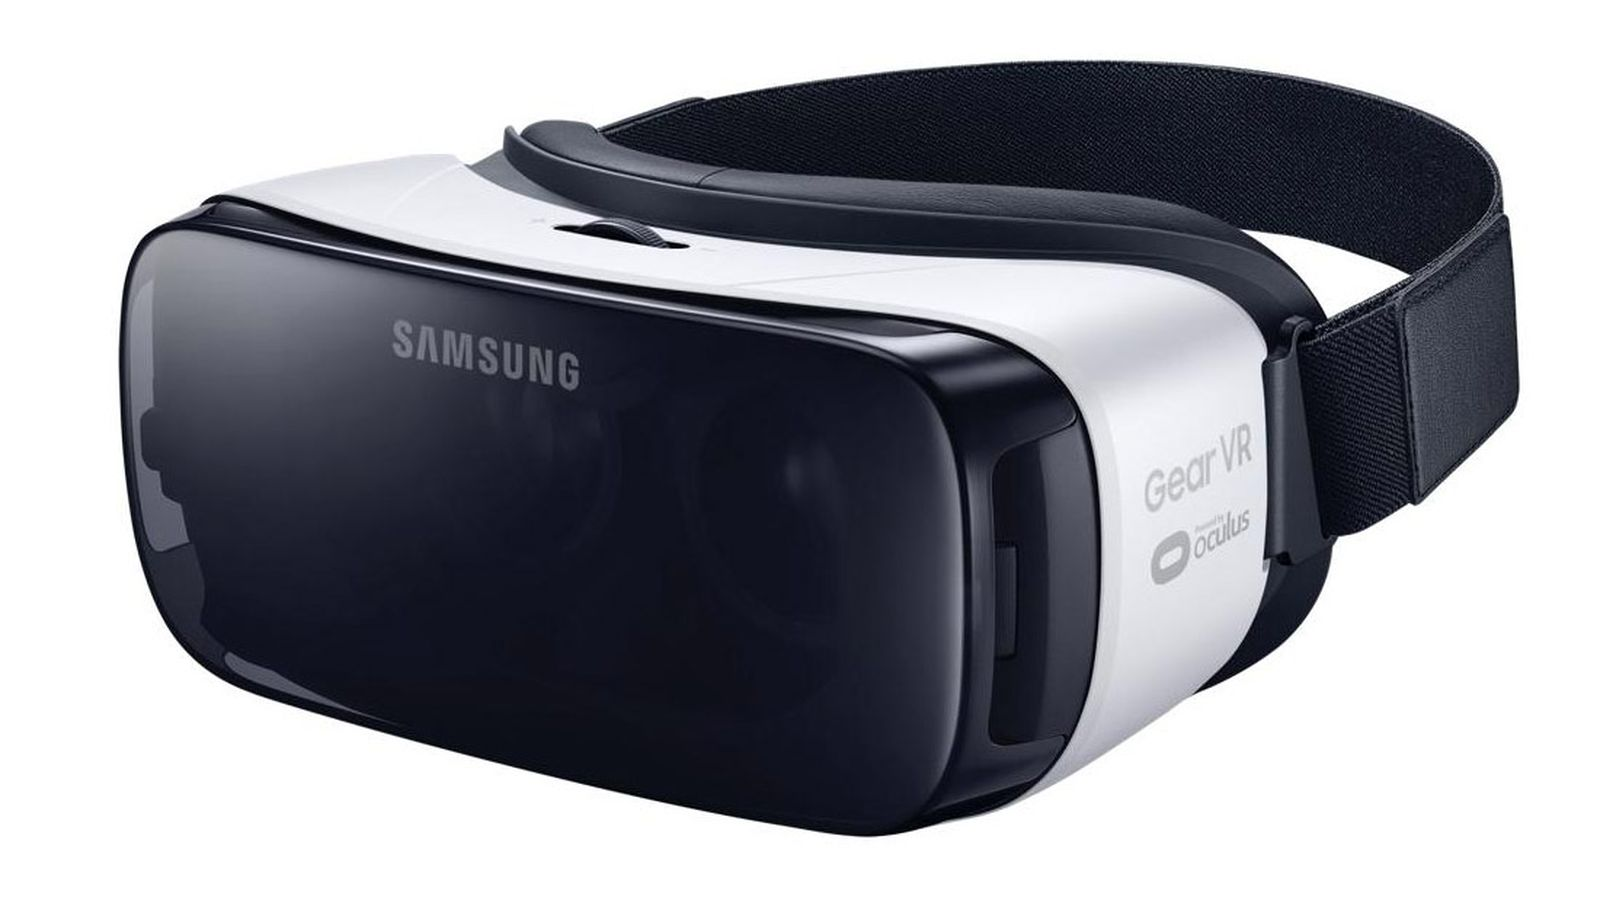
\includegraphics[scale=0.15]{gearvr}
		\caption{Samsung Gear VR}
	\end{center}
\end{figure}
\FloatBarrier

Dopo un periodo di ricerca e \textit{testing} su queste tecnologie, abbiamo deciso di intraprendere la strada \textit{mobile} a discapito di quella desktop. Questa decisione è stata dettata principalmente da due fattori:

\begin{itemize}
	\item \textbf{Requisiti hardware elevati}: per poter offrire un esperienza fluida e piacevole, \textit{Oculus Rift Development kit 2} abbisogna di un PC dall'hardware elevato, non accessibile all'utenza media:
	\begin{itemize}
		\item \textbf{GPU:} NVIDIA GTX 970 / AMD R9 290;
		\item \textbf{CPU:} Intel i5-4590;
		\item \textbf{RAM:} 8GB;
		\item \textbf{Video output:} HDMI 1.3;
		\item \textbf{USB Ports:} 3 porte 3.0 più una porta 2.0;
		\item \textbf{OS:} Windows 7 SP1 64 bit o superiore.
	\end{itemize}
	
	\item \textbf{Obiettivi aziendali:} nonostante fin da subito mi sia stato chiarito che non veniva preteso alcun prodotto finale utilizzabile, l'azienda sperava però di riuscire, con questo stage, a sviluppare un primo prototipo di \textit{virtual showroom} da poter mostrare alle fiere tecnologiche alle quali partecipa. In quest'ottica, l'utilizzo di \textit{Oculus Rift Development kit 2} sarebbe risultato troppo scomodo sia per il trasporto e l'installazione, che per l'utilizzatore finale.
\end{itemize}

Abbiamo deciso, dunque, di sviluppare sia per \textit{Samsung Gear VR} che per \textit{Google Cardboard}, entrambi dispositivi \textit{mobile} a costo contenuto. La progettazione iniziale prevedeva di sviluppare codice che fosse il più possibile indipendente dalla specifica piattaforma, così da creare un unico progetto sia per \textit{Samsung Gear VR} che per \textit{Google Cardboard}. Purtroppo, dopo uno studio più approfondito, questo non fu pienamente possibile poiché gli \textit{SDK}\ped{\hyperlink{sdk}{G}} forniti rispettivamente da Smasung e Google sono profondamente differenti, le metodologie di implementazione degli oggetti interattivi cambiano da una piattaforma all'altra e l'interfaccia per interazione offerta dai due dispositivi è diversa: 

\begin{itemize}
	\item \textbf{Samsung Gear VR} fornisce all'utilizzatore un \textit{touch pad} per selezionare oggetti interattivi e scorrere del testo e un tasto indietro per tornare alla scena o pagina precedente;
	\item \textbf{Google Cardboard} permette all'utilizzatore solamente di selezionare un oggetto attraverso lo spostamento di un magnete come è visibile in figura \hyperlink{gc}{figura 1.9}.
\end{itemize}

La sezione 3.5.1 parla in maniera approfondita della progettazione, delle scelte e dei compromessi che abbiamo dovuto adottare per rendere il progetto il più possibile indipendente dalla piattaforma. \\
Riguardo allo stack software, alla fine della prima settimana di ricerca è andato delineandosi dome segue:

\begin{itemize}
	\item Per lo sviluppo dell'ambiente tridimensionale e del comportamento degli oggetti presenti in esso ho scelto di utilizzare il \textit{framework}\ped{\hyperlink{fw}{G}} \textbf{Unity}. \textit{Unity} è uno strumento di \textit{authoring}\ped{\hyperlink{auth}{G}} integrato e multi-piattaforma per la creazione di videogiochi 3D o altri contenuti interattivi, quali visualizzazioni architettoniche o animazioni in tempo reale. Permette di modellare ambienti e oggetti 3D tramite un editor, fornendo strumenti per modificarne la forma, il colore, posizione e l'interazione con gli altri oggetti e l'ambiente come la forza di gravità, la collisione e molto altro. Per ogni oggetto, offre la possibilità di definirne anche un comportamento attraverso script che andranno agganciati allo stesso. I linguaggi offerti da \textit{Unity} per la composizione degli script sono \textit{JavaScritp} e \textit{C\#}. Entrambi i linguaggi offrono le stesse potenzialità e sul piano prestazionale sono allo stesso livello. Ho deciso però di scegliere \textit{C\#} poiché è risultato essere il più utilizzato all'interno della \textit{community} \textit{Unity};

	\item Per interfacciarsi con il visore, Samsung e Google mettono a disposizione degli \textbf{\textit{SDK}\ped{\hyperlink{sdk}{G}}} dedicati e particolari oggetti \textit{Unity} per l'esperienza \textit{VR}\ped{\hyperlink{vr}{G}}. Gli \textit{SDK}\ped{\hyperlink{sdk}{G}} permettono, negli script, di utilizzare alcuni metodi per catturare l'interazione con l'interfaccia fisica del visore, come la selezione e lo scorrimento del testo. La sezione 3.5.4 parla in maniera approfondita dell'utilizzo di questi metodi e di come sia possibile rendere interattivo un oggetto. Per quanto riguarda gli oggetti \textit{VR}\ped{\hyperlink{vr}{G}} forniti, il più importante e fondamentale tra questi è la \textit{Camera VR}. In \textit{Unity} ogni scena possiede una o più camere che definiscono il punto di vista dell'utente. Una normale camera creata all'interno dell'ambiente non permette l'esperienza \textit{VR}\ped{\hyperlink{vr}{G}}, non essendo collegata ai sensori di inclinazione e spostamento del visore, nel caso di \textit{Samasung Gear VR}, o del telefono, nel caso di \textit{Google Cardboard}. Una volta inserita nella scena la \textit{Camera VR} specifica per ogni piattaforma, essa permette fin da subito la visualizzazione a 360 gradi. Gli \textit{SDK}\ped{\hyperlink{sdk}{G}} e gli oggetti vengono forniti tramite un particolare pacchetto dall'estensione \textit{.unity} da importare nel proprio progetto;

	\item Per sperimentare l'interazione dell'applicazione con sistemi \textit{cloud} esterni, dove recuperare e inviare informazioni, il mio tutor aziendale mi ha consigliato l'utilizzo di \textbf{API Gateway} di \textbf{Amazon Web Service}. \textit{API Gateway} è un servizio che permette di definire \textit{endpoint} per le operazioni HTTP, come GET, POST, PUT eccetera, dove la parte \textit{front-end} e la parte \textit{back-end} di un'applicazione possono collegarsi e dialogare fra loro. Dato che lo sviluppo di un \textit{back-end} non faceva parte degli obbiettivi di stage, l'API creata è stata di tipo \textit{mock}. Ciò significa che ogni operazione HTTP effettuata dall'applicazione verso l'API, riceve risposte statiche create all'interno di \textit{API Gateway}. 
\end{itemize}

\label{Stack Gear VR}
\begin{figure}[ht]
	\begin{center}
		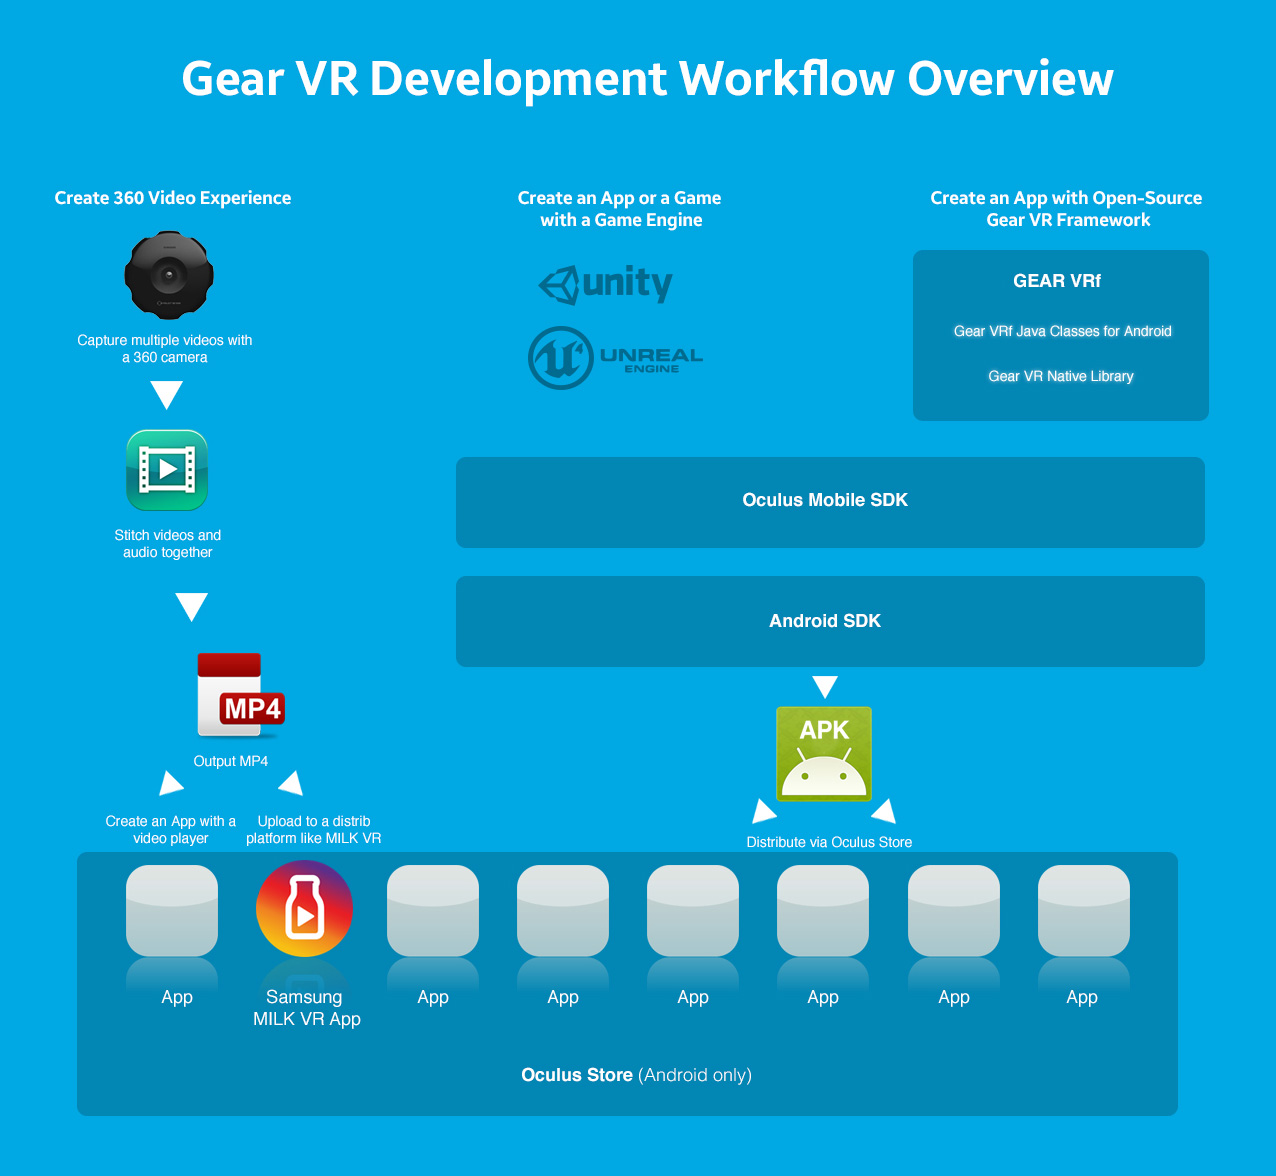
\includegraphics[scale=0.28]{stack-gearvr}
		\caption{Stack tecnologico di sviluppo per Samsung Gear VR. Immagine tratta dal sito SAMSUNG GEAR VR DEVELOPERS US: \url{http://www.samsung.com/us/samsungdeveloperconnection/developer-resources/gear-vr.html}}
	\end{center}
\end{figure}
\FloatBarrier

\subsection{Obiettivi aziendali}

Nel \textit{Piano di Lavoro} presentatomi, l'azienda espone gli obbiettivi minimi e massimi che si aspetta di veder raggiunti alla fine delle 320 ore si stage:

\begin{itemize}
	\item \textbf{Obbiettivi minimi:}
	\begin{enumerate}
		\item Studio delle tecnologie disponibili in ambito \textit{VR}\ped{\hyperlink{vr}{G}} e stesura di un documento riassuntivo che offra un \textit{overview} dello stato attuale della realtà aumentata;
		\item Progettazione e sviluppo di un ambiente virtuale con: una scena e oggetti definiti, un comportamento associato agli oggetti, un prototipo di \textit{user interaction} e scambio di informazioni di base con un sistema di \textit{e-commerce}.
	\end{enumerate}
	\item \textbf{Obbiettivi massimi:}
	\begin{enumerate}
		\item Studio e prototipazione di diversi modelli di \textit{user interaction} con l'ambiente e con gli oggetti finalizzati alla presentazione di un bene vendibile;
		\item Studio e implementazione di possibili nuovi processi di acquisto in ambito \textit{VR}\ped{\hyperlink{vr}{G}}. 
	\end{enumerate}
\end{itemize}

\subsection{Obiettivi personali}

Sono venuto a conoscenza di questo progetto durante l'evento di Stage IT 2016, organizzato da Confindustria Padova in collaborazione con l'Università di Padova e Venezia. Mi ha fin da subito colpito e appassionato per le tecnologie che mi avrebbe permesso di studiare, come ad esempio \textit{Unity}. La computer grafica è da sempre un mio personale interesse e la realtà aumentata è un ambito per me molto affascinante e ricco di opportunità. \\
Le tecnologie proposte dall'azienda purtroppo non rientrano nel percorso di studi, dunque gli obbiettivi formativi personali che mi sono posto riguardano lo studio e la sperimentazione delle tecnologie, senza pretendere di arrivare ad un risultato non prototipale:

\begin{itemize}
	\item \textbf{Obiettivi minimi:}
	\begin{enumerate}
		\item Conoscenza ad alto livello delle tecnologie (hardware e software) attualmente disponibili nel mercato atte a creare ambienti virtuali;
		\item Conoscenza ad alto livello dei concetti principali di \textit{e-commerce} e relative tecnologie di riferimento usate per la vendita online.
	\end{enumerate}
	\item \textbf{Obiettivi massimi:}
	\begin{enumerate}
		\item Capacità di identificare, progettare e sviluppare ambienti virtuali, selezionando le tecnologie attualmente disponibili più appropriate per il caso d'uso;
		\item Presa di coscienza dei concetti multi-channel e omni-channel e come le nuove modalità di vendita si integrino con questi modelli emergenti.
	\end{enumerate}
\end{itemize}